\chapter{検証ライブラリActario}
\label{chapter:overview}

本章では、本研究で作成したアクターシステムの検証ライブラリであるActarioについての概要を説明する。
Actarioでは、

\section{概要}

図\ref{img:overview:workflow}は、Actarioを用いてアクターシステムを検証する際のワークフローである。
まずActarioが提供するアクターシステムを記述するための記法を使って、検証したいアクターシステムを記述する。
次にそのアクターシステムが満たしているべき仕様を記述し、それをActarioが提供する証明の機構によって証明する。
最後にActarioが持つErlangへのコード抽出機を用いて実装をErlangに抽出する。

\begin{figure}[tp]
  \centering
  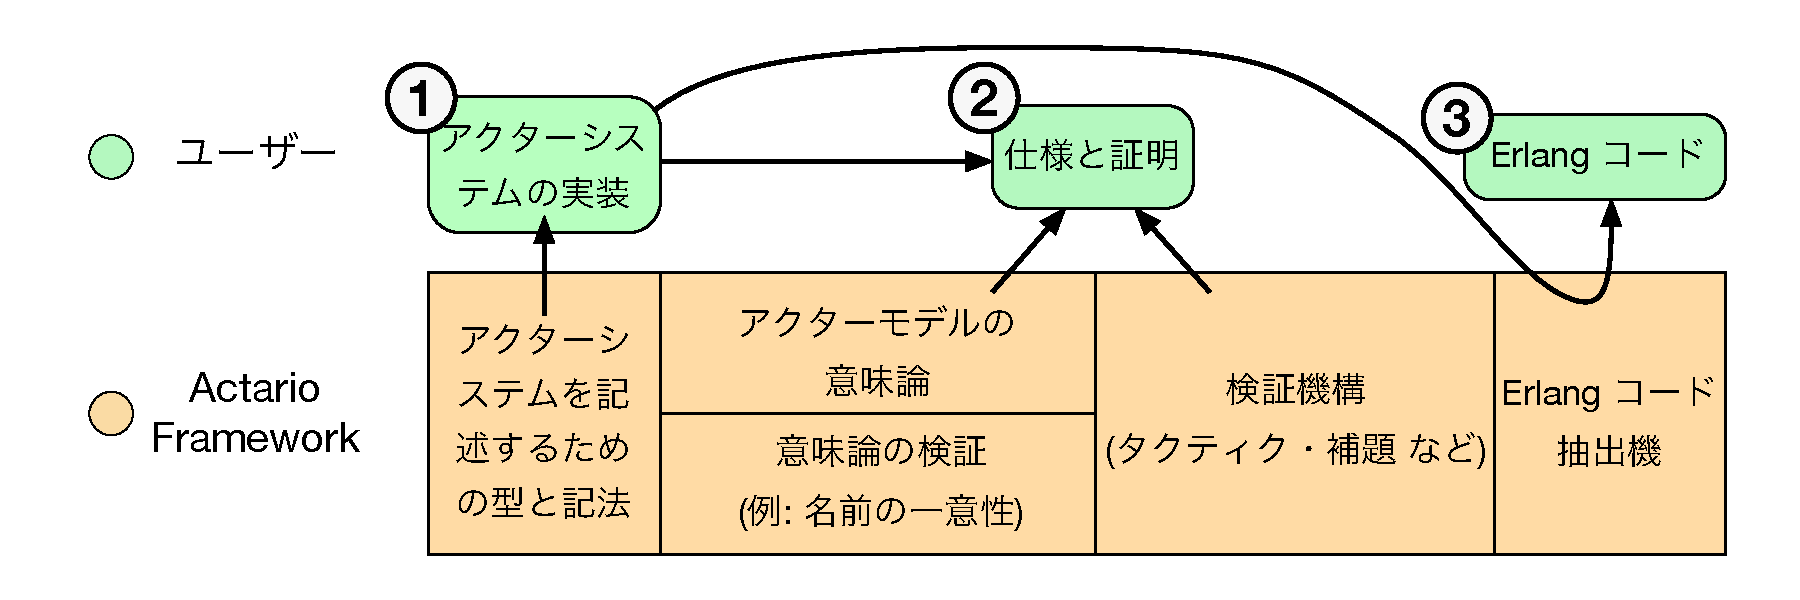
\includegraphics[width=15cm]{./img/overview/workflow.pdf}
  \label{img:overview:workflow}
  \caption{Actarioのワークフロー}
\end{figure}

\section{例:階乗計算アクターシステム}

例として、階乗を計算するアクターシステムを考える。
このシステムをActarioで記述し、仕様および証明を記述することで、
Actarioを実際にどのように使うかを説明する。

\subsection{システムの実装}

このアクターシステムは、単に一つのアクターのなかで階乗を計算するのではなく、
次に何の数を掛けるかという継続を持っているアクターを生成しながら、
階乗を計算する。(?)
図~\ref{img:overview:fact}はこのアクターシステムに$3$を与えたときの動きを表した図である。

\begin{figure}[tp]
  \centering
  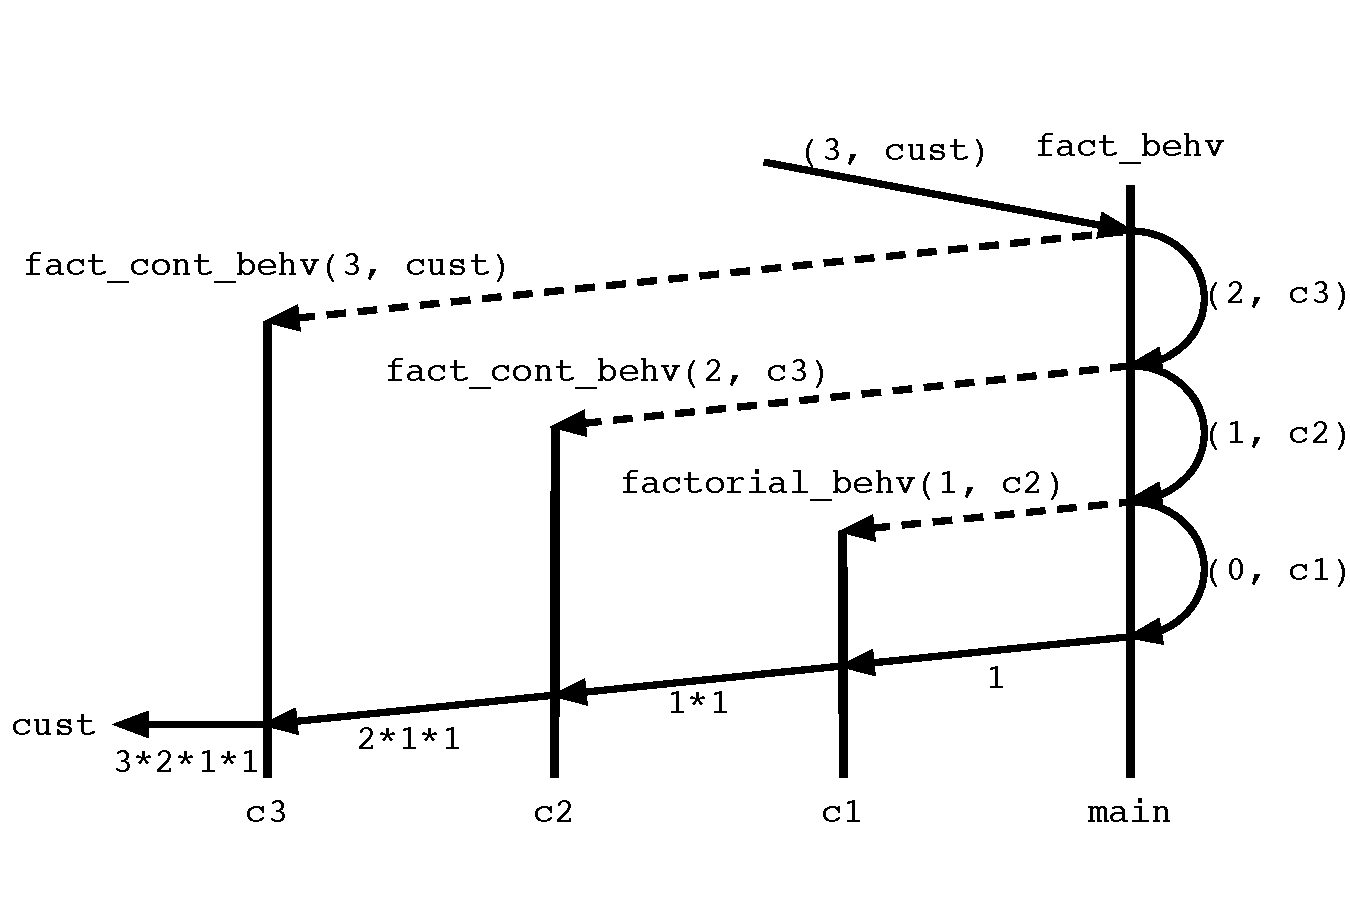
\includegraphics[width=15cm]{./img/overview/fact.pdf}
  \label{img:overview:fact}
  \caption{fact 3}
\end{figure}

Actarioを用いると階乗計算アクターシステムは図~\ref{code:overview:fact-impl}のように記述することができる。
\texttt{factorial\_cont\_behv}は継続を保持しているアクターの振る舞いのテンプレートである。
保持する数と計算結果を渡すアクターの名前を受け取り、アクターの振る舞いとなる。
このアクターは、メッセージを受け取った際にそれが数なら保持している数\texttt{val}と掛けあわせ、
計算結果を待ち受けているアクター\texttt{cust}に送信する。
送信後は何もしないアクターとなる。
次の\texttt{factorial\_behv}は、継続となるアクターを順々に生成していくアクターの振る舞いである。
このアクターは、メッセージを受け取った際に、それが数とアクターの名前の組であり、かつ数が$0$ならば...
最後の\texttt{factorial\_system}はこのアクターシステムを起動する部分(?)である。

\begin{figure}[tp]
  \lstinputlisting{./code/overview/fact_impl.v}
  \label{code:overview:fact-impl}
  \caption{階乗計算アクターシステム}
\end{figure}

\subsection{命題の定義と証明}

また、証明の例として、「このアクターシステムは3の階乗を計算する」ということを証明する。
3の階乗を計算するということはつまりメッセージとして送られた自然数$3$に対して、$3!$を返信するということなので、
命題は図\ref{code:overview:fact-spec}のように記述することができる。これは、$3$を階乗計算システムに送信すると、トップレベルアクターはいつか$6$を受け取るという意味である。

\begin{figure}[tp]
\begin{lstlisting}
Theorem receive_3 :
  eventually_receive (factorial_system 3 top) top (nat_msg 6).
\end{lstlisting}
\label{code:overview:fact-spec}
\caption{命題の定義}
\end{figure}

そして、この命題は図~\ref{code:overview:fact-proof}のように証明することができる。
証明の方針としては、遷移を一つずつ追っていき、トップレベルアクターが$6$を受け取るような遷移を見つけるというものである。遷移できなくなるまで遷移の生成はActarioが提供するタクティクが行う。

\begin{figure}[tp]
\begin{lstlisting}
Proof.
  unfold_eventually eventually_receive=> p p0 is_path.
  step_until_stop is_path p0.
  finish 22 p22 p23.
Qed.
\end{lstlisting}
  \label{code:overview:fact-proof}
  \caption{証明}
\end{figure}


\subsection{Erlangへのコード抽出}

ActarioはErlangへのコード抽出機構も持っているため、
定義したアプリケーションをErlangに変換して実行させることもできる。
図\ref{code:overview:extraction}のコマンドを実行すると、\coqi{factorial_behv}のErlang実装が\texttt{factorial.erl}というファイル名で吐き出される。
これに対して、図\ref{code:overview:run}といったようなコードで変換されたアクターシステムを起動させると、実際にアクターシステムを実行することができる。

\begin{figure}[tp]
\begin{lstlisting}
ActorExtraction "factorial" factorial_behv.
\end{lstlisting}
\label{code:overview:extraction}
\caption{証明}
\end{figure}

\begin{figure}
\begin{lstlisting}
-module(fact_main).
-export([fact/1]).

fact(N) ->
    FactorialActor = spawn(fun() -> factorial:factorial_behv({tt}) end),
    FactorialActor ! {tuple_msg, {nat_msg, int2nat(N)}, {name_msg, self()}},
    receive
        {nat_msg, Result} ->
            io:fwrite("fact(~w) = ~w~n", [N, nat2int(Result)]);
        _ ->
            io:fwrite("error~n")
    end.

nat2int({o}) -> 0;
nat2int({s, N}) -> nat2int(N) + 1.

int2nat(0) -> {o};
int2nat(N) when N > 0 -> {s, int2nat(N - 1)};
int2nat(_) -> {o}.
\end{lstlisting}
\label{code:overview:run}
\caption{証明}
\end{figure}
